\section{Bee Colony Algorithm}

\begin{figure}[h]
	\centering
	\begin{subfigure}{.5\textwidth}
		\centering
		\captionsetup{width=0.75\linewidth}
		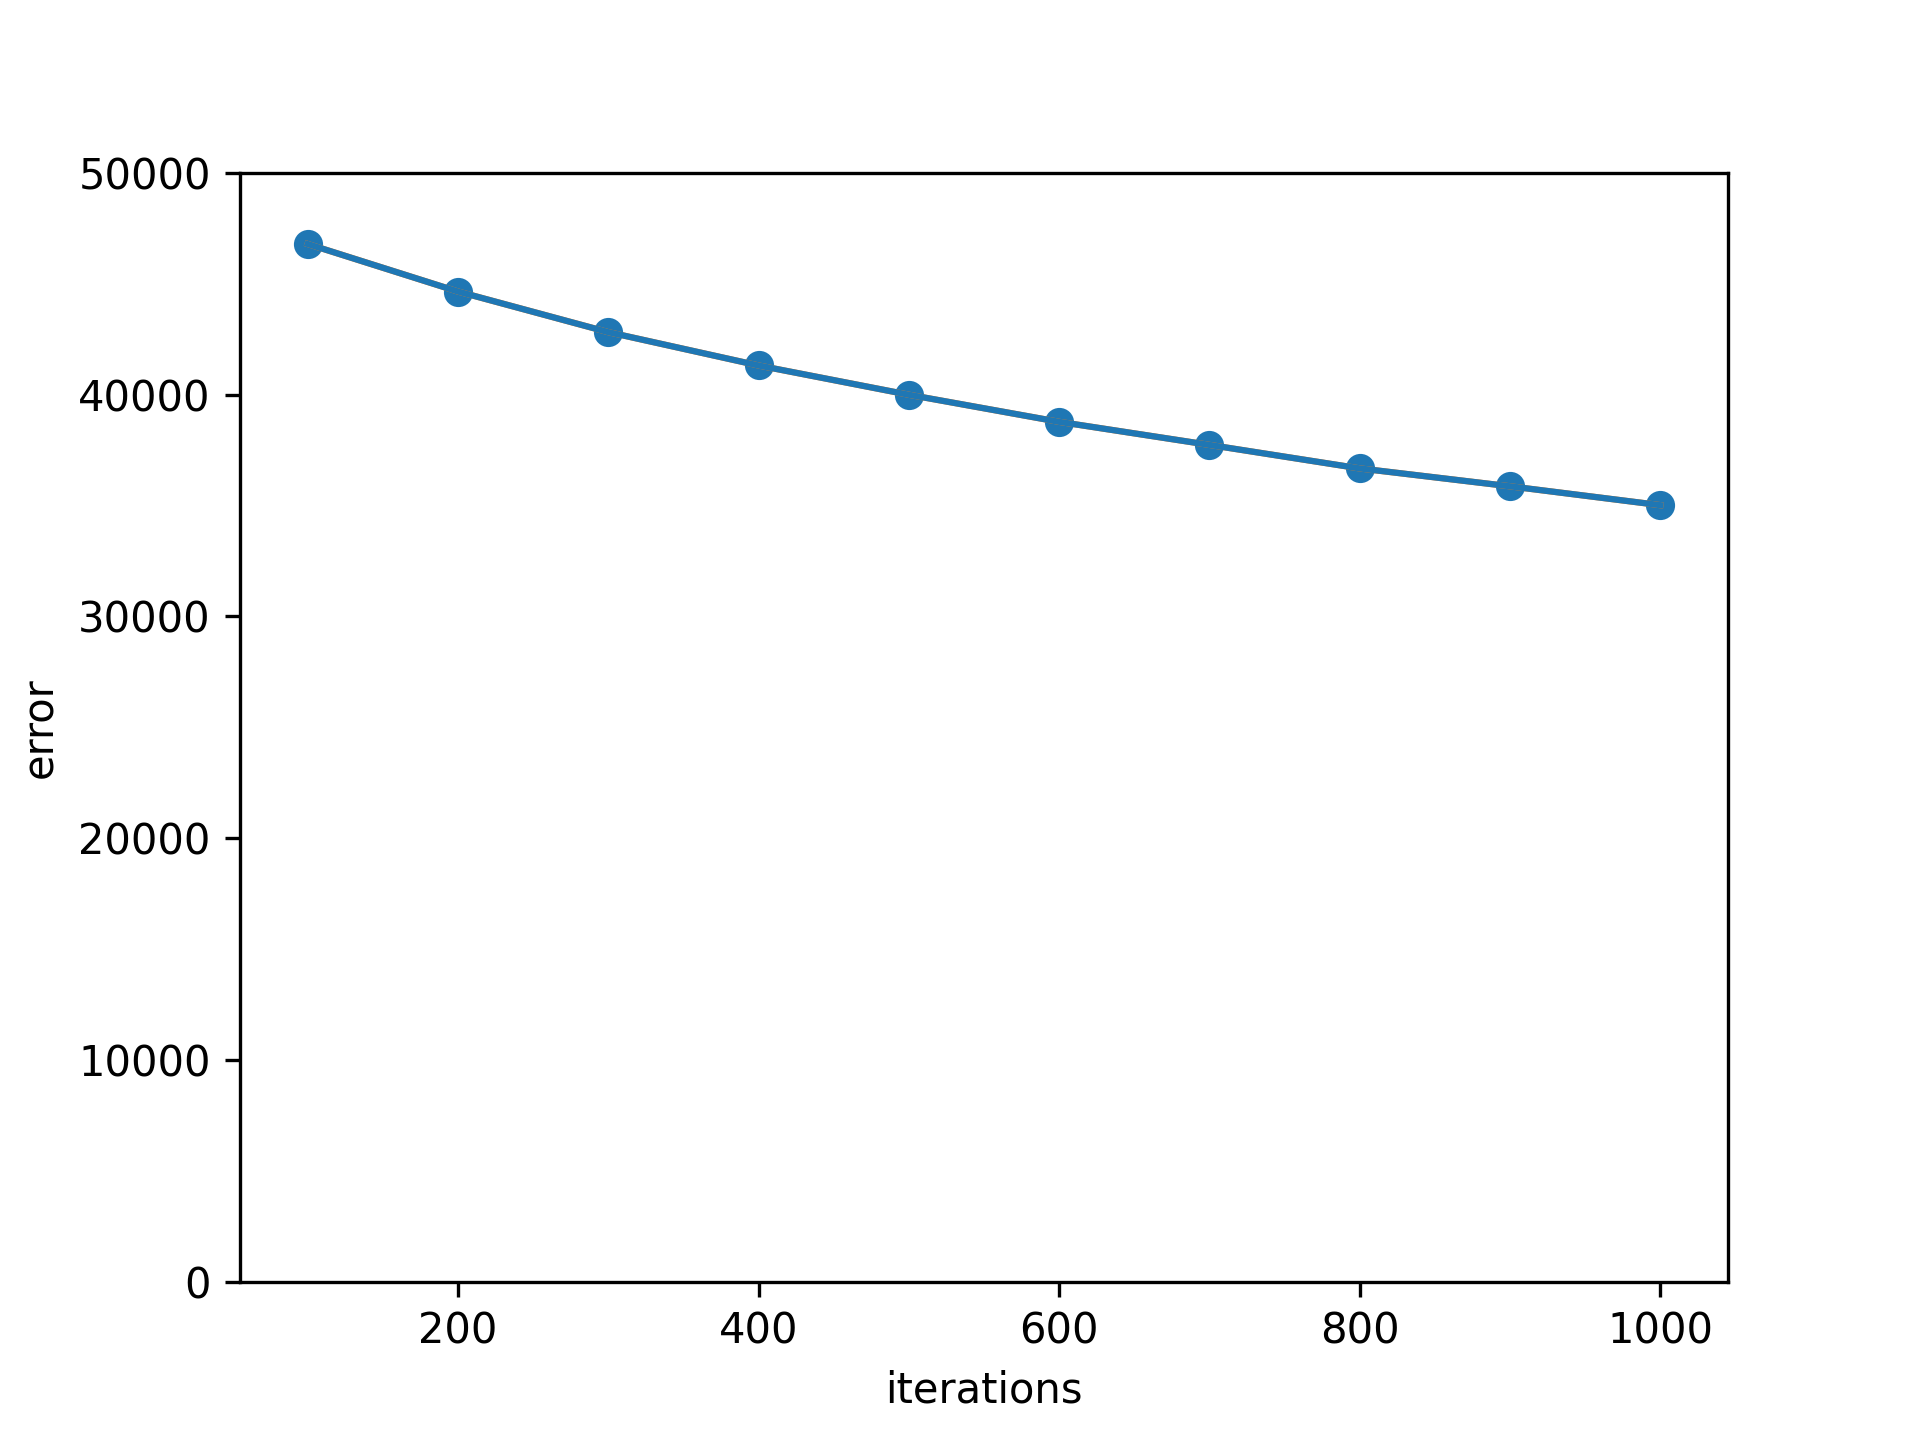
\includegraphics[width=0.75\linewidth]{assets/reference_tsp.png}
		\caption{Error over iterations using the reference evolutionary algorithm.}
		\label{fig:reference_tsp}
	\end{subfigure}%
	\begin{subfigure}{.5\textwidth}
		\centering
    \captionsetup{width=0.75\linewidth}
		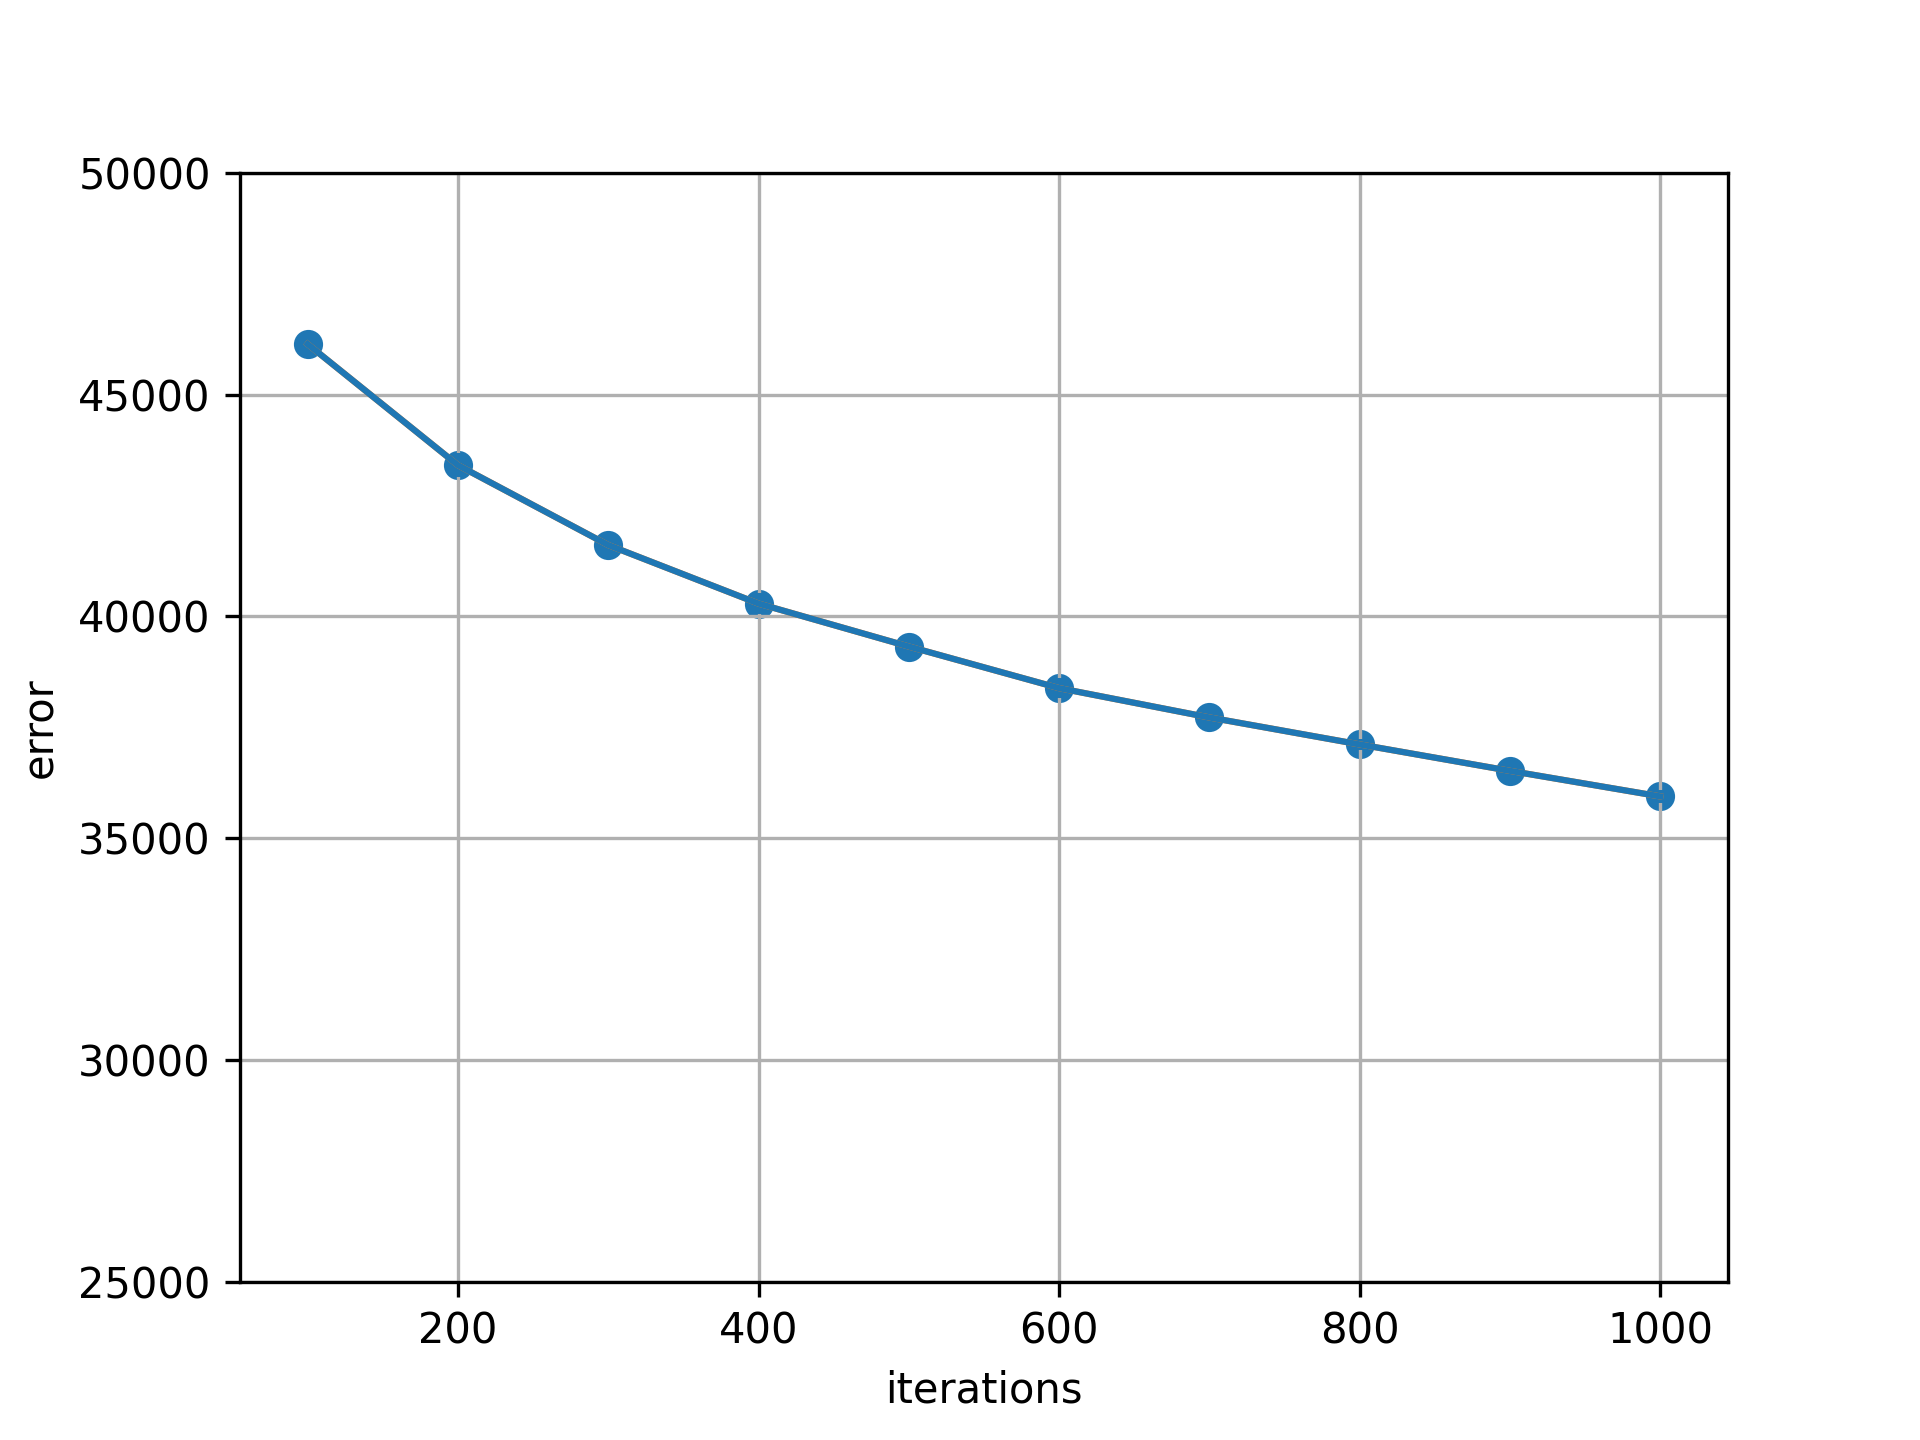
\includegraphics[width=0.75\linewidth]{assets/beecolony_tsp.png}
		\caption{Error over iterations using the bee colony algorithm.}
		\label{fig:becolony_tsp}
	\end{subfigure}
	\caption{Comparison of bee colony and evolutionary algorithm on the TSP problem.}
	\label{fig:bee_vs_ea}
\end{figure}

\begin{table}[H]
	\centering
	\begin{tabular}{|c c c c|}
		\hline
		\textbf{Optimizer} & \textbf{Error} & \textbf{Evaluations} & \textbf{Runtime [s]} \\
		\hline
		Bee Colony Algorithm & $37380.08 \pm 213.10$ & 100050 & 3.75 \\
		Reference Evolutionary Algorithm & $35012.41 \pm 482.07$ & 25000 & 2.90 \\
		\hline
	\end{tabular}
	\caption{Minimal errors after the given number of evaluations produced by optimisers on the TSP problem. Results are averaged over 10 subsequent runs.}
	\label{tab:bee_vs_ea}
\end{table}
